\documentclass[11pt,a4paper]{article}
\usepackage[utf8]{inputenc}
\usepackage[T1]{fontenc}
\usepackage[margin=0.7in]{geometry}
\usepackage{booktabs}
\usepackage{array}
\usepackage{longtable}
\usepackage{amsmath}
\usepackage{amssymb}
\usepackage{pgfplots}
\pgfplotsset{compat=1.18}
\usepgfplotslibrary{statistics}
\usetikzlibrary{patterns}

% Black-and-white only — no colour anywhere. Strict line-based visual rhythm.
\definecolor{linegray}{HTML}{222222}

\title{Eigen vs numpy state-vector: 80 hard-quantum benchmarks across 23 categories}
\author{Eigen 2.7 hard-quantum benchmark harness}
\date{\today}

\begin{document}
\maketitle

\section{Setup}

For each of 80 hand-written quantum circuits spanning Bell,
GHZ, W-state, Deutsch/Deutsch-Jozsa, Bernstein-Vazirani, Grover (2-5 qubit),
QFT (2-6 qubit), phase estimation, superdense coding, teleportation, Draper
adder, Ising Trotterisation, quantum walk, variational ansatz (VQE-style),
random circuits (3-6 qubit, depth 25-200), Steane \& Shor error-correcting
encoders, and phase-mixer long-depth stress tests,
we execute the \emph{identical EQIR graph} through two paths:
\begin{itemize}
  \item \textbf{Eigen:} \texttt{EigenRuntime} with the Rust-accelerated dense
      state-vector backend
      (\texttt{src.simulator.\allowbreak RustStatevectorWrapper}).
  \item \textbf{numpy:} a textbook matrix-vector simulator in pure
      \texttt{numpy} (no optimisations, no Kronecker trick): every gate is
      applied via \texttt{np.tensordot}/\texttt{transpose}/\texttt{reshape}
      on a dense $2^n$-length state vector.
\end{itemize}
Both sides report the final state vector in the \emph{same} bitstring
convention. Accuracy is reported as $1-\tfrac{1}{2}\sum_b|p^{\text{e}}_b -
p^{\text{n}}_b|$ where $p_b = |\psi_b|^2$ over the union of all basis states.
Speedup $\equiv t_{\text{numpy}}/t_{\text{Eigen}}$; values $>1$ mean Eigen is
faster. \emph{Depth} is the longest chain of qubit-overlapping gates under
topological scheduling.

All timings are best-of-3 after 1 warm-up discarded. The Eigen graph is
\emph{compiled once and re-executed} so the measurement isolates state-vector
evolution (parse / type-check / compile cost is amortised).

\section{Results (long multi-page table)}

\begingroup
\setlength{\tabcolsep}{2pt}
\renewcommand{\arraystretch}{0.96}
\tiny
\begin{longtable}{@{}>{\raggedright\arraybackslash}p{4.0cm} >{\raggedright\arraybackslash}p{1.7cm} r r r r r r r r r@{}}
\caption{Hard-quantum head-to-head over all 80 test cases.
$Q$ = qubits, $g$ = gates, $d$=depth. \texttt{PASS} requires accuracy $\ge 99.9\%$.
\textbf{80 pass / 0 fail}.}\\
\toprule
Test case & cat & $\mathbf{q}$ & $\mathbf{g}$ & $\mathbf{d}$ & Eigen (ms) & numpy (ms) & speedup & acc (\%) & max dev & status \\
\midrule[0.4pt]
\endfirsthead
\multicolumn{11}{c}{\tiny\itshape continued from previous page}\\
\toprule
Test case & cat & $\mathbf{q}$ & $\mathbf{g}$ & $\mathbf{d}$ & Eigen (ms) & numpy (ms) & speedup & acc (\%) & max dev & status \\
\midrule[0.4pt]
\endhead
\midrule[0.1pt]
\multicolumn{11}{r}{\tiny\itshape continued on next page}\\
\endfoot
\midrule[0.4pt]
\textbf{mean (over valid rows)} & -- & -- & -- & -- & 0.127 & 0.367 & 2.89 & 100.0000 & 7.90e-16 & -- \\
\bottomrule
\endlastfoot
01\_bell\_phi\_plus & Bell & 2 & 2 & 2 & 0.04 & 0.029 & 0.73 & 100.0000 & 2.22e-16 & PASS \\
\midrule[0.1pt]
02\_bell\_psi\_plus & Bell & 2 & 3 & 3 & 0.04 & 0.034 & 0.86 & 100.0000 & 2.22e-16 & PASS \\
\midrule[0.1pt]
03\_bell\_phi\_minus & Bell & 2 & 3 & 3 & 0.04 & 0.034 & 0.84 & 100.0000 & 2.22e-16 & PASS \\
\midrule[0.1pt]
04\_ghz\_3 & GHZ & 3 & 3 & 3 & 0.04 & 0.041 & 0.98 & 100.0000 & 2.22e-16 & PASS \\
\midrule[0.1pt]
05\_ghz\_5 & GHZ & 5 & 5 & 5 & 0.06 & 0.071 & 1.26 & 100.0000 & 2.22e-16 & PASS \\
\midrule[0.1pt]
06\_w\_state\_3 & W-state & 3 & 5 & 5 & 0.05 & 0.068 & 1.31 & 100.0000 & 0.00e+00 & PASS \\
\midrule[0.1pt]
07\_deutsch\_balanced & Deutsch & 2 & 6 & 4 & 0.04 & 0.052 & 1.25 & 100.0000 & 1.11e-15 & PASS \\
\midrule[0.1pt]
08\_deutsch\_jozsa\_balanced\_3 & Deutsch-Jozsa & 3 & 8 & 5 & 0.05 & 0.074 & 1.50 & 100.0000 & 6.11e-16 & PASS \\
\midrule[0.1pt]
09\_bernstein\_vazirani\_101 & BV & 4 & 10 & 5 & 0.06 & 0.094 & 1.65 & 100.0000 & 7.77e-16 & PASS \\
\midrule[0.1pt]
10\_grover\_2q\_marked\_11 & Grover & 2 & 12 & 7 & 0.05 & 0.101 & 2.01 & 100.0000 & 1.33e-15 & PASS \\
\midrule[0.1pt]
11\_grover\_3q\_marked\_101 & Grover & 3 & 46 & 22 & 0.11 & 0.340 & 3.20 & 100.0000 & 3.33e-15 & PASS \\
\midrule[0.1pt]
12\_qft\_3\_on\_001 & QFT & 3 & 8 & 6 & 0.06 & 0.109 & 1.75 & 100.0000 & 8.33e-17 & PASS \\
\midrule[0.1pt]
13\_qft\_4\_on\_1101 & QFT & 4 & 15 & 9 & 0.09 & 0.201 & 2.22 & 100.0000 & 9.71e-17 & PASS \\
\midrule[0.1pt]
14\_phase\_estimation\_quarter & QPE & 4 & 13 & 8 & 0.07 & 0.163 & 2.18 & 100.0000 & 1.44e-15 & PASS \\
\midrule[0.1pt]
15\_superdense\_coding\_00 & Superdense & 2 & 4 & 4 & 0.04 & 0.041 & 1.04 & 100.0000 & 8.88e-16 & PASS \\
\midrule[0.1pt]
16\_superdense\_coding\_10 & Superdense & 2 & 5 & 5 & 0.04 & 0.047 & 1.14 & 100.0000 & 8.88e-16 & PASS \\
\midrule[0.1pt]
17\_quantum\_walk\_cycle4\_4step & Quantum walk & 3 & 13 & 13 & 0.06 & 0.147 & 2.27 & 100.0000 & 6.11e-16 & PASS \\
\midrule[0.1pt]
18\_ising\_3\_trotter & Ising-Trotter & 3 & 28 & 26 & 0.10 & 0.279 & 2.79 & 100.0000 & 1.94e-16 & PASS \\
\midrule[0.1pt]
19\_draper\_adder\_1plus1 & Draper & 4 & 12 & 10 & 0.07 & 0.150 & 2.15 & 100.0000 & 3.33e-16 & PASS \\
\midrule[0.1pt]
20\_grover\_4q\_marked\_1000 & Grover & 5 & 100 & 37 & 0.21 & 0.837 & 3.92 & 100.0000 & 9.77e-15 & PASS \\
\midrule[0.1pt]
21\_bell\_psi\_minus & Bell & 2 & 4 & 3 & 0.04 & 0.042 & 1.03 & 100.0000 & 2.22e-16 & PASS \\
\midrule[0.1pt]
22\_ghz\_2 & GHZ & 2 & 2 & 2 & 0.04 & 0.027 & 0.74 & 100.0000 & 2.22e-16 & PASS \\
\midrule[0.1pt]
23\_ghz\_7 & GHZ & 7 & 7 & 7 & 0.09 & 0.115 & 1.29 & 100.0000 & 2.22e-16 & PASS \\
\midrule[0.1pt]
24\_ghz\_10 & GHZ & 10 & 10 & 10 & 0.40 & 0.340 & 0.85 & 100.0000 & 2.22e-16 & PASS \\
\midrule[0.1pt]
25\_w\_state\_5 & W-state & 5 & 14 & 7 & 0.10 & 0.181 & 1.79 & 100.0000 & 6.94e-18 & PASS \\
\midrule[0.1pt]
26\_deutsch\_constant & Deutsch & 2 & 4 & 2 & 0.04 & 0.036 & 0.90 & 100.0000 & 4.44e-16 & PASS \\
\midrule[0.1pt]
27\_deutsch\_jozsa\_constant\_3 & Deutsch-Jozsa & 3 & 6 & 2 & 0.05 & 0.052 & 1.13 & 100.0000 & 6.11e-16 & PASS \\
\midrule[0.1pt]
28\_bv\_110 & BV & 4 & 10 & 5 & 0.06 & 0.095 & 1.67 & 100.0000 & 7.77e-16 & PASS \\
\midrule[0.1pt]
29\_bv\_011 & BV & 4 & 10 & 5 & 0.06 & 0.093 & 1.63 & 100.0000 & 7.77e-16 & PASS \\
\midrule[0.1pt]
30\_bv\_111 & BV & 4 & 11 & 6 & 0.06 & 0.104 & 1.76 & 100.0000 & 7.77e-16 & PASS \\
\midrule[0.1pt]
31\_grover\_2q\_marked\_00 & Grover & 2 & 16 & 9 & 0.06 & 0.124 & 2.22 & 100.0000 & 1.33e-15 & PASS \\
\midrule[0.1pt]
32\_grover\_2q\_marked\_01 & Grover & 2 & 14 & 9 & 0.05 & 0.109 & 2.08 & 100.0000 & 1.33e-15 & PASS \\
\midrule[0.1pt]
33\_grover\_2q\_marked\_10 & Grover & 2 & 14 & 9 & 0.05 & 0.111 & 2.09 & 100.0000 & 1.33e-15 & PASS \\
\midrule[0.1pt]
34\_grover\_3q\_marked\_000 & Grover & 3 & 27 & 13 & 0.08 & 0.200 & 2.45 & 100.0000 & 2.00e-15 & PASS \\
\midrule[0.1pt]
35\_grover\_3q\_marked\_010 & Grover & 3 & 25 & 13 & 0.08 & 0.186 & 2.37 & 100.0000 & 2.00e-15 & PASS \\
\midrule[0.1pt]
36\_grover\_3q\_marked\_111 & Grover & 3 & 21 & 11 & 0.07 & 0.164 & 2.25 & 100.0000 & 2.22e-15 & PASS \\
\midrule[0.1pt]
37\_grover\_4q\_marked\_0101 & Grover & 5 & 34 & 13 & 0.12 & 0.313 & 2.67 & 100.0000 & 1.67e-15 & PASS \\
\midrule[0.1pt]
38\_grover\_4q\_marked\_1111 & Grover & 5 & 30 & 11 & 0.11 & 0.284 & 2.56 & 100.0000 & 1.83e-15 & PASS \\
\midrule[0.1pt]
39\_grover\_5q\_marked\_00000 & Grover & 7 & 49 & 17 & 0.20 & 0.543 & 2.72 & 100.0000 & 9.99e-16 & PASS \\
\midrule[0.1pt]
40\_grover\_5q\_marked\_11111 & Grover & 7 & 39 & 15 & 0.18 & 0.478 & 2.59 & 100.0000 & 9.99e-16 & PASS \\
\midrule[0.1pt]
41\_qft\_2\_on\_01 & QFT & 2 & 5 & 4 & 0.05 & 0.062 & 1.34 & 100.0000 & 2.22e-16 & PASS \\
\midrule[0.1pt]
42\_qft\_5\_on\_10101 & QFT & 5 & 20 & 11 & 0.13 & 0.302 & 2.25 & 100.0000 & 6.59e-17 & PASS \\
\midrule[0.1pt]
43\_qft\_6\_on\_100100 & QFT & 6 & 26 & 13 & 0.21 & 0.464 & 2.25 & 100.0000 & 4.51e-17 & PASS \\
\midrule[0.1pt]
44\_qpe\_half & QPE & 4 & 14 & 8 & 0.08 & 0.184 & 2.17 & 100.0000 & 6.11e-16 & PASS \\
\midrule[0.1pt]
45\_qpe\_eighth & QPE & 4 & 14 & 8 & 0.09 & 0.184 & 2.15 & 100.0000 & 1.33e-15 & PASS \\
\midrule[0.1pt]
46\_qpe\_quarter\_4ancilla & QPE & 5 & 21 & 10 & 0.12 & 0.293 & 2.51 & 100.0000 & 5.00e-16 & PASS \\
\midrule[0.1pt]
47\_superdense\_coding\_01 & Superdense & 2 & 5 & 5 & 0.04 & 0.050 & 1.17 & 100.0000 & 8.88e-16 & PASS \\
\midrule[0.1pt]
48\_superdense\_coding\_11 & Superdense & 2 & 6 & 6 & 0.04 & 0.054 & 1.23 & 100.0000 & 8.88e-16 & PASS \\
\midrule[0.1pt]
49\_teleport\_zero & Teleport & 3 & 6 & 6 & 0.05 & 0.099 & 1.94 & 100.0000 & 2.22e-16 & PASS \\
\midrule[0.1pt]
50\_teleport\_superposed & Teleport & 3 & 8 & 6 & 0.06 & 0.100 & 1.64 & 100.0000 & 1.11e-16 & PASS \\
\midrule[0.1pt]
51\_steane\_encoder\_0L & Steane-QEC & 7 & 17 & 7 & 0.11 & 0.219 & 2.00 & 100.0000 & 1.78e-15 & PASS \\
\midrule[0.1pt]
52\_shor\_encoder\_0L & Shor-QEC & 9 & 9 & 5 & 0.20 & 0.240 & 1.19 & 100.0000 & 2.22e-16 & PASS \\
\midrule[0.1pt]
53\_vqe\_h2\_4q\_2layer & VQE & 4 & 24 & 12 & 0.12 & 0.279 & 2.32 & 100.0000 & 1.11e-16 & PASS \\
\midrule[0.1pt]
54\_vqe\_5q\_4layer & VQE & 5 & 60 & 28 & 0.22 & 0.704 & 3.17 & 100.0000 & 6.94e-17 & PASS \\
\midrule[0.1pt]
55\_vqe\_3q\_6layer & VQE & 3 & 54 & 30 & 0.16 & 0.537 & 3.27 & 100.0000 & 1.11e-16 & PASS \\
\midrule[0.1pt]
56\_random\_4q\_d50 & Random & 4 & 50 & 31 & 0.15 & 0.489 & 3.27 & 100.0000 & 4.44e-16 & PASS \\
\midrule[0.1pt]
57\_random\_5q\_d30 & Random & 5 & 30 & 15 & 0.12 & 0.315 & 2.53 & 100.0000 & 2.50e-16 & PASS \\
\midrule[0.1pt]
58\_random\_3q\_d100 & Random & 3 & 100 & 65 & 0.23 & 0.932 & 4.08 & 100.0000 & 2.00e-15 & PASS \\
\midrule[0.1pt]
59\_random\_6q\_d25 & Random & 6 & 25 & 11 & 0.13 & 0.307 & 2.41 & 100.0000 & 9.71e-17 & PASS \\
\midrule[0.1pt]
60\_random\_4q\_d200 & Random & 4 & 200 & 128 & 0.41 & 1.913 & 4.71 & 100.0000 & 7.22e-16 & PASS \\
\midrule[0.1pt]
61\_ising\_30\_trotter\_5step & Ising-Trotter & 3 & 33 & 31 & 0.11 & 0.335 & 3.11 & 100.0000 & 1.25e-16 & PASS \\
\midrule[0.1pt]
62\_ising\_30\_trotter\_10step & Ising-Trotter & 3 & 63 & 61 & 0.16 & 0.620 & 3.76 & 100.0000 & 1.11e-16 & PASS \\
\midrule[0.1pt]
63\_ising\_30\_trotter\_25step & Ising-Trotter & 3 & 153 & 151 & 0.35 & 1.510 & 4.36 & 100.0000 & 1.25e-16 & PASS \\
\midrule[0.1pt]
64\_ising\_30\_trotter\_50step & Ising-Trotter & 3 & 303 & 301 & 0.61 & 3.079 & 5.06 & 100.0000 & 1.25e-16 & PASS \\
\midrule[0.1pt]
65\_ising\_30\_trotter\_100step & Ising-Trotter & 3 & 603 & 601 & 1.17 & 5.870 & 5.04 & 100.0000 & 1.11e-16 & PASS \\
\midrule[0.1pt]
66\_draper\_adder\_2plus2 & Draper & 4 & 13 & 12 & 0.07 & 0.158 & 2.22 & 100.0000 & 1.33e-15 & PASS \\
\midrule[0.1pt]
67\_draper\_adder\_3plus5 & Draper & 6 & 24 & 17 & 0.12 & 0.330 & 2.81 & 100.0000 & 9.99e-16 & PASS \\
\midrule[0.1pt]
68\_draper\_adder\_4plus4 & Draper & 6 & 22 & 18 & 0.11 & 0.313 & 2.73 & 100.0000 & 1.22e-15 & PASS \\
\midrule[0.1pt]
69\_draper\_adder\_7plus1 & Draper & 6 & 24 & 18 & 0.12 & 0.345 & 2.91 & 100.0000 & 9.99e-16 & PASS \\
\midrule[0.1pt]
70\_quantum\_walk\_8step & Quantum walk & 3 & 25 & 25 & 0.09 & 0.271 & 2.98 & 100.0000 & 9.44e-16 & PASS \\
\midrule[0.1pt]
71\_quantum\_walk\_16step & Quantum walk & 3 & 49 & 49 & 0.12 & 0.488 & 3.96 & 100.0000 & 1.55e-15 & PASS \\
\midrule[0.1pt]
72\_qft\_5\_on\_00000 & QFT & 5 & 17 & 10 & 0.13 & 0.262 & 2.10 & 100.0000 & 9.02e-17 & PASS \\
\midrule[0.1pt]
73\_ghz\_6\_alt\_staircase & GHZ & 6 & 7 & 7 & 0.07 & 0.100 & 1.38 & 100.0000 & 2.22e-16 & PASS \\
\midrule[0.1pt]
74\_clifford\_t\_staircase & Clifford+T & 3 & 8 & 6 & 0.06 & 0.076 & 1.38 & 100.0000 & 2.78e-16 & PASS \\
\midrule[0.1pt]
75\_ghz\_4\_with\_ry\_phase & GHZ & 4 & 6 & 5 & 0.06 & 0.078 & 1.35 & 100.0000 & 1.11e-16 & PASS \\
\midrule[0.1pt]
76\_cry\_crx\_chain\_3q & CRY/CRX & 3 & 6 & 5 & 0.06 & 0.087 & 1.51 & 100.0000 & 2.22e-16 & PASS \\
\midrule[0.1pt]
77\_8q\_phase\_mixer & Phase mixer & 8 & 19 & 9 & 0.57 & 0.699 & 1.23 & 100.0000 & 7.81e-18 & PASS \\
\midrule[0.1pt]
78\_bell\_chain\_with\_swap & Bell chain & 3 & 5 & 5 & 0.05 & 0.061 & 1.32 & 100.0000 & 2.22e-16 & PASS \\
\midrule[0.1pt]
79\_phase\_chain\_8 & Phase chain & 4 & 14 & 9 & 0.09 & 0.187 & 2.08 & 100.0000 & 1.11e-16 & PASS \\
\midrule[0.1pt]
80\_quantum\_walk\_damped\_coin\_6step & Quantum walk & 3 & 25 & 25 & 0.09 & 0.285 & 3.12 & 100.0000 & 1.05e-15 & PASS \\
\end{longtable}
\endgroup

\section{Per-category aggregation}

\begin{table}[h]
\centering
\small
\setlength{\tabcolsep}{4pt}
\renewcommand{\arraystretch}{1.05}
\begin{tabular}{@{}l r r r r r r r r@{}}
\toprule
Category & $n$ & mean $\mathbf{q}$ & mean $\mathbf{g}$ & mean $\mathbf{d}$ & Eigen (ms) & numpy (ms) & mean sp & mean acc (\%) \\
\midrule[0.4pt]
Ising-Trotter & 6 & 3.0 & 197.2 & 195.2 & 0.415 & 1.949 & 4.69 & 100.0000 \\
Random & 5 & 4.4 & 81.0 & 50.0 & 0.207 & 0.791 & 3.82 & 100.0000 \\
VQE & 3 & 4.0 & 46.0 & 23.3 & 0.169 & 0.507 & 3.00 & 100.0000 \\
Grover & 13 & 3.8 & 32.8 & 14.3 & 0.106 & 0.292 & 2.75 & 100.0000 \\
Quantum walk & 4 & 3.0 & 28.0 & 28.0 & 0.093 & 0.298 & 3.21 & 100.0000 \\
Draper & 5 & 5.2 & 19.0 & 15.0 & 0.098 & 0.259 & 2.64 & 100.0000 \\
Phase mixer & 1 & 8.0 & 19.0 & 9.0 & 0.569 & 0.699 & 1.23 & 100.0000 \\
Steane-QEC & 1 & 7.0 & 17.0 & 7.0 & 0.110 & 0.219 & 2.00 & 100.0000 \\
QPE & 4 & 4.2 & 15.5 & 8.5 & 0.090 & 0.206 & 2.28 & 100.0000 \\
QFT & 6 & 4.2 & 15.2 & 8.8 & 0.111 & 0.233 & 2.11 & 100.0000 \\
Phase chain & 1 & 4.0 & 14.0 & 9.0 & 0.090 & 0.187 & 2.08 & 100.0000 \\
BV & 4 & 4.0 & 10.2 & 5.2 & 0.057 & 0.097 & 1.68 & 100.0000 \\
W-state & 2 & 4.0 & 9.5 & 6.0 & 0.077 & 0.124 & 1.63 & 100.0000 \\
Shor-QEC & 1 & 9.0 & 9.0 & 5.0 & 0.203 & 0.240 & 1.19 & 100.0000 \\
Clifford+T & 1 & 3.0 & 8.0 & 6.0 & 0.055 & 0.076 & 1.38 & 100.0000 \\
Deutsch-Jozsa & 2 & 3.0 & 7.0 & 3.5 & 0.048 & 0.063 & 1.32 & 100.0000 \\
Teleport & 2 & 3.0 & 7.0 & 6.0 & 0.056 & 0.099 & 1.78 & 100.0000 \\
CRY/CRX & 1 & 3.0 & 6.0 & 5.0 & 0.058 & 0.087 & 1.51 & 100.0000 \\
GHZ & 7 & 5.3 & 5.7 & 5.6 & 0.108 & 0.110 & 1.02 & 100.0000 \\
Deutsch & 2 & 2.0 & 5.0 & 3.0 & 0.040 & 0.044 & 1.08 & 100.0000 \\
Superdense & 4 & 2.0 & 5.0 & 5.0 & 0.042 & 0.048 & 1.15 & 100.0000 \\
Bell chain & 1 & 3.0 & 5.0 & 5.0 & 0.047 & 0.061 & 1.32 & 100.0000 \\
Bell & 4 & 2.0 & 3.0 & 2.8 & 0.040 & 0.035 & 0.87 & 100.0000 \\
\\ \midrule[0.4pt]
\textbf{overall} & 80 & -- & -- & -- & 0.127 & 0.367 & 2.89 & 100.0000 \\
\bottomrule
\end{tabular}
\caption{Per-category aggregation: each row summarises one category of tests.
Categories sorted by descending mean gate count (largest circuits first).}
\end{table}

\section{Speed comparison (log scale)}

\begin{figure}[h]
\centering
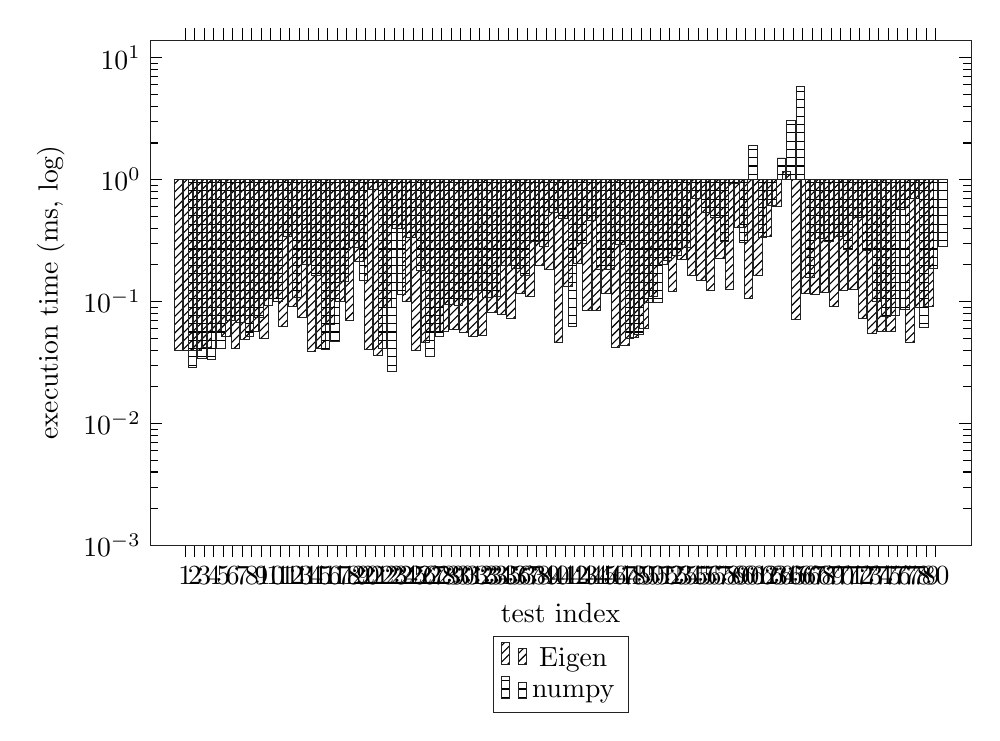
\begin{tikzpicture}
\begin{axis}[
    width=0.99\textwidth,
    height=8cm,
    ybar,
    bar width=3pt,
    enlarge x limits=0.04,
    ymin=0.001,
    ymode=log,
    ytick={0.001, 0.01, 0.1, 1, 10, 100, 1000},
    ylabel={execution time (ms, log)},
    xlabel={test index},
    legend style={at={(0.5,-0.18)},anchor=north,draw=linegray},
    every axis/.append style={draw=linegray, very thin},
    every tick/.append style={black, thin},
    every axis label/.append style={black},
    xtick={1,2,3,4,5,6,7,8,9,10,11,12,13,14,15,16,17,18,19,20,21,22,23,24,25,26,27,28,29,30,31,32,33,34,35,36,37,38,39,40,41,42,43,44,45,46,47,48,49,50,51,52,53,54,55,56,57,58,59,60,61,62,63,64,65,66,67,68,69,70,71,72,73,74,75,76,77,78,79,80},
    xmin=0.5, xmax=80.5,
]
\addplot+[draw=linegray, fill=lightgray!50, pattern=north east lines, mark=none]
    coordinates { (1,0.0398) (2,0.0397) (3,0.0401) (4,0.0423) (5,0.0563) (6,0.0521) (7,0.0414) (8,0.0494) (9,0.0568) (10,0.0501) (11,0.1065) (12,0.0623) (13,0.0908) (14,0.0747) (15,0.0394) (16,0.0415) (17,0.0647) (18,0.0999) (19,0.0699) (20,0.2137) (21,0.0406) (22,0.0366) (23,0.0890) (24,0.4003) (25,0.1011) (26,0.0396) (27,0.0461) (28,0.0570) (29,0.0570) (30,0.0591) (31,0.0559) (32,0.0522) (33,0.0534) (34,0.0816) (35,0.0787) (36,0.0729) (37,0.1171) (38,0.1108) (39,0.1994) (40,0.1845) (41,0.0463) (42,0.1341) (43,0.2059) (44,0.0848) (45,0.0856) (46,0.1168) (47,0.0425) (48,0.0439) (49,0.0509) (50,0.0608) (51,0.1100) (52,0.2027) (53,0.1204) (54,0.2223) (55,0.1639) (56,0.1493) (57,0.1245) (58,0.2284) (59,0.1272) (60,0.4058) (61,0.1074) (62,0.1649) (63,0.3463) (64,0.6087) (65,1.1656) (66,0.0712) (67,0.1174) (68,0.1145) (69,0.1183) (70,0.0911) (71,0.1233) (72,0.1251) (73,0.0723) (74,0.0552) (75,0.0576) (76,0.0576) (77,0.5695) (78,0.0466) (79,0.0899) (80,0.0914) };
\addplot+[draw=linegray, fill=lightgray!10, pattern=horizontal lines, mark=none]
    coordinates { (1,0.0291) (2,0.0340) (3,0.0338) (4,0.0414) (5,0.0708) (6,0.0680) (7,0.0517) (8,0.0742) (9,0.0936) (10,0.1008) (11,0.3404) (12,0.1091) (13,0.2015) (14,0.1632) (15,0.0409) (16,0.0472) (17,0.1468) (18,0.2786) (19,0.1505) (20,0.8370) (21,0.0417) (22,0.0270) (23,0.1152) (24,0.3398) (25,0.1810) (26,0.0358) (27,0.0519) (28,0.0954) (29,0.0930) (30,0.1043) (31,0.1241) (32,0.1085) (33,0.1114) (34,0.1998) (35,0.1864) (36,0.1639) (37,0.3126) (38,0.2838) (39,0.5430) (40,0.4780) (41,0.0622) (42,0.3019) (43,0.4638) (44,0.1837) (45,0.1838) (46,0.2928) (47,0.0497) (48,0.0539) (49,0.0989) (50,0.0996) (51,0.2195) (52,0.2403) (53,0.2795) (54,0.7036) (55,0.5365) (56,0.4887) (57,0.3149) (58,0.9317) (59,0.3067) (60,1.9130) (61,0.3345) (62,0.6195) (63,1.5100) (64,3.0794) (65,5.8705) (66,0.1581) (67,0.3303) (68,0.3126) (69,0.3445) (70,0.2711) (71,0.4878) (72,0.2621) (73,0.0998) (74,0.0761) (75,0.0777) (76,0.0869) (77,0.6986) (78,0.0615) (79,0.1871) (80,0.2852) };
\legend{Eigen, numpy}
\end{axis}
\end{tikzpicture}
\caption{Best-of-3 execution time per test. Log scale so the 1-2-qubit Bell
tests ($\sim$40 µs) coexist in the same axes with the longest Trotter /
random-circuit tests.}
\end{figure}

\section{Accuracy per test}

\begin{figure}[h]
\centering
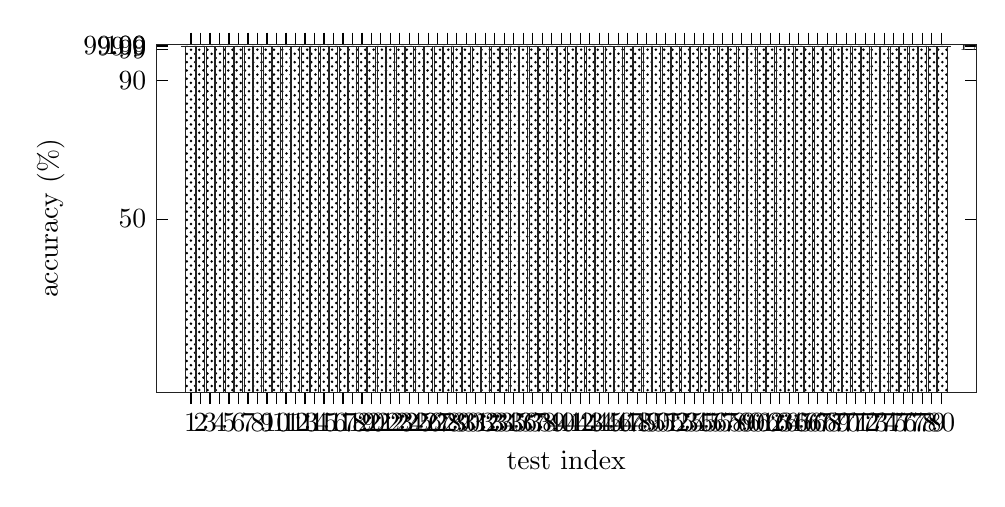
\begin{tikzpicture}
\begin{axis}[
    width=0.99\textwidth,
    height=6cm,
    ybar,
    bar width=4pt,
    enlarge x limits=0.04,
    ymin=0.0,
    ymax=100.4,
    ytick={50, 90, 99, 99.9, 99.99, 100},
    ylabel={accuracy (\%)},
    xlabel={test index},
    legend style={at={(0.5,-0.18)},anchor=north,draw=linegray},
    every axis/.append style={draw=linegray, very thin},
    every tick/.append style={black, thin},
    every axis label/.append style={black},
    xtick={1,2,3,4,5,6,7,8,9,10,11,12,13,14,15,16,17,18,19,20,21,22,23,24,25,26,27,28,29,30,31,32,33,34,35,36,37,38,39,40,41,42,43,44,45,46,47,48,49,50,51,52,53,54,55,56,57,58,59,60,61,62,63,64,65,66,67,68,69,70,71,72,73,74,75,76,77,78,79,80},
    xmin=0.5, xmax=80.5,
]
\addplot+[draw=linegray, fill=lightgray!40, pattern=crosshatch dots, mark=none]
    coordinates { (1,100.0000) (2,100.0000) (3,100.0000) (4,100.0000) (5,100.0000) (6,100.0000) (7,100.0000) (8,100.0000) (9,100.0000) (10,100.0000) (11,100.0000) (12,100.0000) (13,100.0000) (14,100.0000) (15,100.0000) (16,100.0000) (17,100.0000) (18,100.0000) (19,100.0000) (20,100.0000) (21,100.0000) (22,100.0000) (23,100.0000) (24,100.0000) (25,100.0000) (26,100.0000) (27,100.0000) (28,100.0000) (29,100.0000) (30,100.0000) (31,100.0000) (32,100.0000) (33,100.0000) (34,100.0000) (35,100.0000) (36,100.0000) (37,100.0000) (38,100.0000) (39,100.0000) (40,100.0000) (41,100.0000) (42,100.0000) (43,100.0000) (44,100.0000) (45,100.0000) (46,100.0000) (47,100.0000) (48,100.0000) (49,100.0000) (50,100.0000) (51,100.0000) (52,100.0000) (53,100.0000) (54,100.0000) (55,100.0000) (56,100.0000) (57,100.0000) (58,100.0000) (59,100.0000) (60,100.0000) (61,100.0000) (62,100.0000) (63,100.0000) (64,100.0000) (65,100.0000) (66,100.0000) (67,100.0000) (68,100.0000) (69,100.0000) (70,100.0000) (71,100.0000) (72,100.0000) (73,100.0000) (74,100.0000) (75,100.0000) (76,100.0000) (77,100.0000) (78,100.0000) (79,100.0000) (80,100.0000) };
\draw [linegray, dashed, very thin] (axis cs:0,99.9) -- (axis cs:81,99.9)
    node [linegray, anchor=west, font=\tiny] at (axis cs:81, 99.9) {PASS line};
\end{axis}
\end{tikzpicture}
\caption{Accuracy per test. Anything below the 99.9\,\% line fails the
comparison. The bar is clamped to the 0-100.4\,\% window.}
\end{figure}

\section{Speedup histogram}

\begin{figure}[h]
\centering
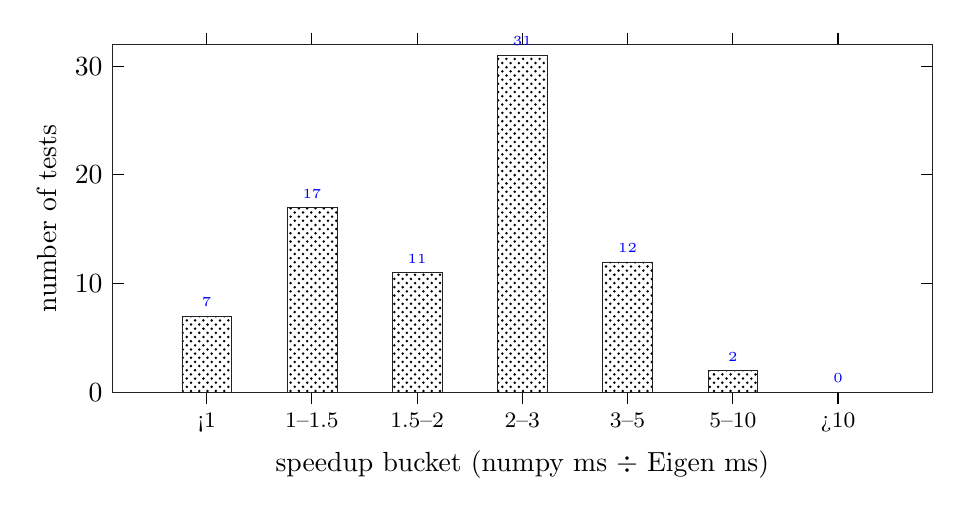
\begin{tikzpicture}
\begin{axis}[
    width=0.99\textwidth,
    height=6cm,
    ybar,
    bar width=18pt,
    enlarge x limits=0.15,
    ymin=0,
    ylabel={number of tests},
    xlabel={speedup bucket (numpy ms $\div$ Eigen ms)},
    every axis/.append style={draw=linegray, very thin},
    every tick/.append style={black, thin},
    every axis label/.append style={black},
    nodes near coords,
    nodes near coords style={font=\tiny},
    xtick={1,2,3,4,5,6,7},
    xticklabels={<1, 1--1.5, 1.5--2, 2--3, 3--5, 5--10, >10},
    xticklabel style={font=\footnotesize},
    ymin=0, ymax=32,
]
\addplot+[draw=linegray, fill=lightgray!40, pattern=crosshatch dots, mark=none]
    coordinates { (1,7) (2,17) (3,11) (4,31) (5,12) (6,2) (7,0) };
\end{axis}
\end{tikzpicture}
\caption{How speedups distribute across all 80 tests.
A speedup $<1$ means numpy was faster than Eigen on that test; $>1$ means
Eigen's Rust backend won.}
\end{figure}

\section{Quadrant (4-field matrix): log-scale gates $\times$ qubits}

\begin{figure}[h]
\centering
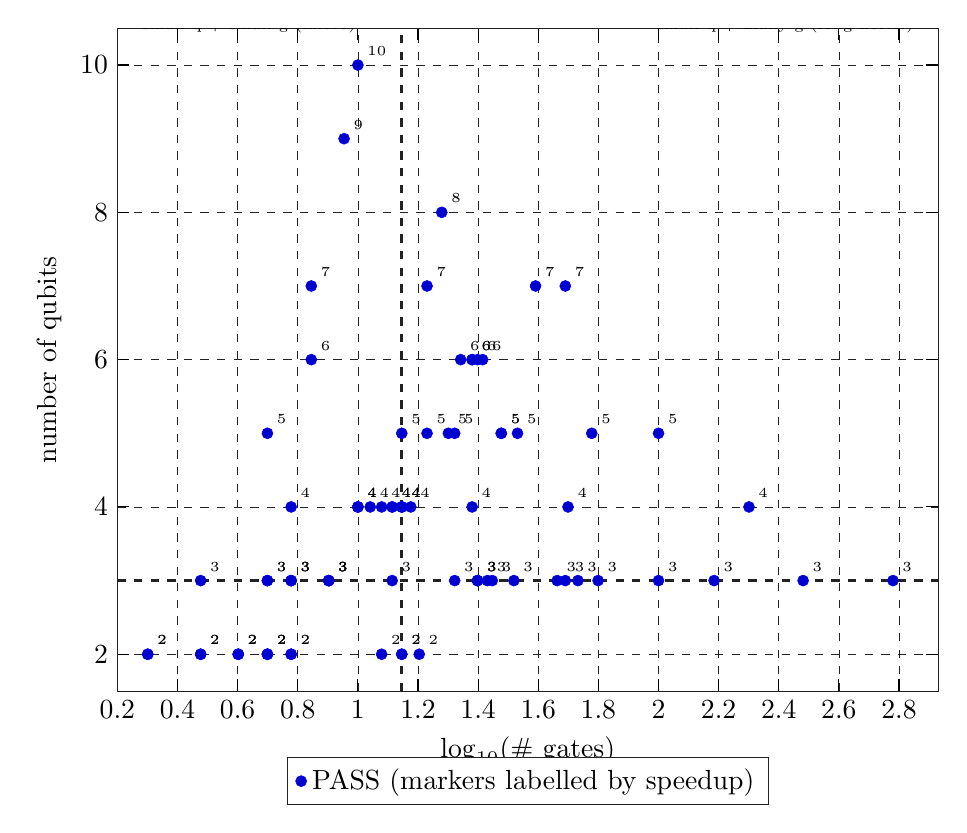
\begin{tikzpicture}
\begin{axis}[
    width=0.99\textwidth,
    height=10cm,
    xlabel={$\log_{10}(\text{\# gates})$},
    ylabel={number of qubits},
    grid=major,
    grid style={linegray, very thin, dashed},
    every axis/.append style={draw=linegray, very thin},
    every tick/.append style={black, thin},
    every axis label/.append style={black},
    legend style={at={(0.5,-0.10)},anchor=north,draw=linegray,fill=white},
    legend entries={PASS (markers labelled by speedup), FAIL},
    xmin=0.20, xmax=2.93,
    ymin=1.5, ymax=10.5,
]
\addplot+[only marks, mark=*, mark size=2pt,
    nodes near coords={\tiny \pgfmathprintnumber[fixed,precision=2]{\pgfplotspointmeta}},
    nodes near coords style={font=\tiny, anchor=south west, black}
]
    coordinates { (0.301,2)[0.73] (0.477,2)[0.86] (0.477,2)[0.84] (0.477,3)[0.98] (0.699,5)[1.26] (0.699,3)[1.31] (0.778,2)[1.25] (0.903,3)[1.50] (1.000,4)[1.65] (1.079,2)[2.01] (1.663,3)[3.20] (0.903,3)[1.75] (1.176,4)[2.22] (1.114,4)[2.18] (0.602,2)[1.04] (0.699,2)[1.14] (1.114,3)[2.27] (1.447,3)[2.79] (1.079,4)[2.15] (2.000,5)[3.92] (0.602,2)[1.03] (0.301,2)[0.74] (0.845,7)[1.29] (1.000,10)[0.85] (1.146,5)[1.79] (0.602,2)[0.90] (0.778,3)[1.13] (1.000,4)[1.67] (1.000,4)[1.63] (1.041,4)[1.76] (1.204,2)[2.22] (1.146,2)[2.08] (1.146,2)[2.09] (1.431,3)[2.45] (1.398,3)[2.37] (1.322,3)[2.25] (1.531,5)[2.67] (1.477,5)[2.56] (1.690,7)[2.72] (1.591,7)[2.59] (0.699,2)[1.34] (1.301,5)[2.25] (1.415,6)[2.25] (1.146,4)[2.17] (1.146,4)[2.15] (1.322,5)[2.51] (0.699,2)[1.17] (0.778,2)[1.23] (0.778,3)[1.94] (0.903,3)[1.64] (1.230,7)[2.00] (0.954,9)[1.19] (1.380,4)[2.32] (1.778,5)[3.17] (1.732,3)[3.27] (1.699,4)[3.27] (1.477,5)[2.53] (2.000,3)[4.08] (1.398,6)[2.41] (2.301,4)[4.71] (1.519,3)[3.11] (1.799,3)[3.76] (2.185,3)[4.36] (2.481,3)[5.06] (2.780,3)[5.04] (1.114,4)[2.22] (1.380,6)[2.81] (1.342,6)[2.73] (1.380,6)[2.91] (1.398,3)[2.98] (1.690,3)[3.96] (1.230,5)[2.10] (0.845,6)[1.38] (0.903,3)[1.38] (0.778,4)[1.35] (0.778,3)[1.51] (1.279,8)[1.23] (0.699,3)[1.32] (1.146,4)[2.08] (1.398,3)[3.12] };
\addplot+[only marks, mark=triangle, mark size=3pt, draw=black, fill=white]
    coordinates {  };
% Quadrant divider lines at median log10(gates) and median qubits.
\draw [linegray, very thick, dashed] (axis cs:1.146,1.5)
    -- (axis cs:1.146,10.5);
\draw [linegray, very thick, dashed] (axis cs:0.20,3.0)
    -- (axis cs:2.93,3.0);
\node[font=\tiny, anchor=south west, black] at (axis cs:0.25,10.3)
    {small q + small g (micro)};
\node[font=\tiny, anchor=south east, black] at (axis cs:2.88,10.3)
    {small q + many g (long horiz.)};
\node[font=\tiny, anchor=north west, black] at (axis cs:0.25,1.6)
    {many q + small g (tall)};
\node[font=\tiny, anchor=north east, black] at (axis cs:2.88,1.6)
    {many q + many g (extreme)};
\end{axis}
\end{tikzpicture}
\caption{Quadrant (4-field matrix) of test cases. Horizontal axis:
$\log_{10}$ of the gate count, vertical axis: number of qubits. Each
\emph{filled circle} is one PASS test labelled with its speedup (numpy ms
$\div$ Eigen ms). \emph{Hollow triangles} mark FAIL tests. Dashed lines split
the four canonical strategy quadrants: micro (low-q/low-g), long horizontal
(low-q/many-g), tall (many-q/low-g), and extreme (many-q/many-g). The medians
are at $\log_{10} g = 1.15$ and $q = 3.0$.}
\end{figure}

\section{Scaling: runtime vs gate count (log-log)}

\begin{figure}[h]
\centering
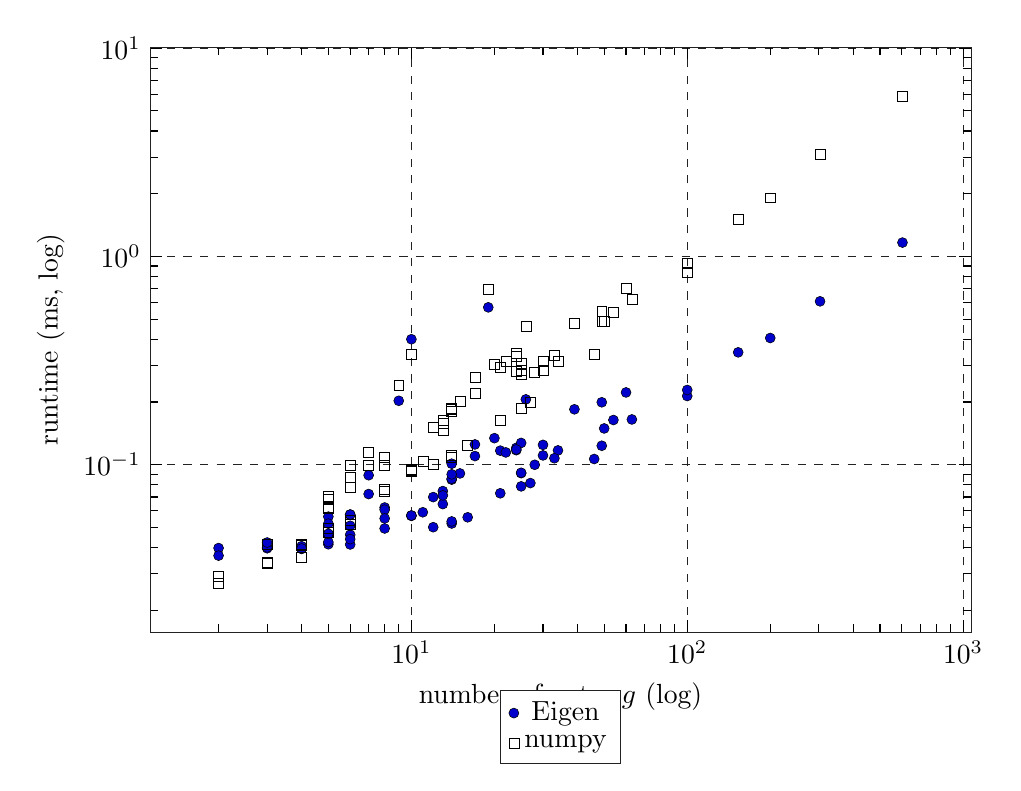
\begin{tikzpicture}
\begin{axis}[
    width=0.99\textwidth,
    height=9cm,
    xmode=log,
    ymode=log,
    log basis x=10,
    log basis y=10,
    xlabel={number of gates $g$ (log)},
    ylabel={runtime (ms, log)},
    grid=major,
    grid style={linegray, very thin, dashed},
    every axis/.append style={draw=linegray, very thin},
    every tick/.append style={black, thin},
    every axis label/.append style={black},
    legend style={at={(0.5,-0.10)},anchor=north,draw=linegray,fill=white},
]
\addplot+[only marks, mark=*, mark size=1.8pt, draw=black, fill=lightgray!50]
    coordinates { (2,0.0398) (3,0.0397) (3,0.0401) (3,0.0423) (5,0.0563) (5,0.0521) (6,0.0414) (8,0.0494) (10,0.0568) (12,0.0501) (46,0.1065) (8,0.0623) (15,0.0908) (13,0.0747) (4,0.0394) (5,0.0415) (13,0.0647) (28,0.0999) (12,0.0699) (100,0.2137) (4,0.0406) (2,0.0366) (7,0.0890) (10,0.4003) (14,0.1011) (4,0.0396) (6,0.0461) (10,0.0570) (10,0.0570) (11,0.0591) (16,0.0559) (14,0.0522) (14,0.0534) (27,0.0816) (25,0.0787) (21,0.0729) (34,0.1171) (30,0.1108) (49,0.1994) (39,0.1845) (5,0.0463) (20,0.1341) (26,0.2059) (14,0.0848) (14,0.0856) (21,0.1168) (5,0.0425) (6,0.0439) (6,0.0509) (8,0.0608) (17,0.1100) (9,0.2027) (24,0.1204) (60,0.2223) (54,0.1639) (50,0.1493) (30,0.1245) (100,0.2284) (25,0.1272) (200,0.4058) (33,0.1074) (63,0.1649) (153,0.3463) (303,0.6087) (603,1.1656) (13,0.0712) (24,0.1174) (22,0.1145) (24,0.1183) (25,0.0911) (49,0.1233) (17,0.1251) (7,0.0723) (8,0.0552) (6,0.0576) (6,0.0576) (19,0.5695) (5,0.0466) (14,0.0899) (25,0.0914) };
\addplot+[only marks, mark=square, mark size=1.8pt, draw=black, fill=white]
    coordinates { (2,0.0291) (3,0.0340) (3,0.0338) (3,0.0414) (5,0.0708) (5,0.0680) (6,0.0517) (8,0.0742) (10,0.0936) (12,0.1008) (46,0.3404) (8,0.1091) (15,0.2015) (13,0.1632) (4,0.0409) (5,0.0472) (13,0.1468) (28,0.2786) (12,0.1505) (100,0.8370) (4,0.0417) (2,0.0270) (7,0.1152) (10,0.3398) (14,0.1810) (4,0.0358) (6,0.0519) (10,0.0954) (10,0.0930) (11,0.1043) (16,0.1241) (14,0.1085) (14,0.1114) (27,0.1998) (25,0.1864) (21,0.1639) (34,0.3126) (30,0.2838) (49,0.5430) (39,0.4780) (5,0.0622) (20,0.3019) (26,0.4638) (14,0.1837) (14,0.1838) (21,0.2928) (5,0.0497) (6,0.0539) (6,0.0989) (8,0.0996) (17,0.2195) (9,0.2403) (24,0.2795) (60,0.7036) (54,0.5365) (50,0.4887) (30,0.3149) (100,0.9317) (25,0.3067) (200,1.9130) (33,0.3345) (63,0.6195) (153,1.5100) (303,3.0794) (603,5.8705) (13,0.1581) (24,0.3303) (22,0.3126) (24,0.3445) (25,0.2711) (49,0.4878) (17,0.2621) (7,0.0998) (8,0.0761) (6,0.0777) (6,0.0869) (19,0.6986) (5,0.0615) (14,0.1871) (25,0.2852) };
\legend{Eigen, numpy}
\end{axis}
\end{tikzpicture}
\caption{Log-log scaling of runtime vs gate count. A clean slope is the
expected power-law $t \sim g^{\alpha}$ with $\alpha\approx 1$ in the regime
where Python overhead per gate dominates over state-vector size work; a
knee above $\sim$ 4-5 qubits reveals the denser matrix-vs-vector cost.}
\end{figure}

\section{Accuracy error magnitude vs gate count}

\begin{figure}[h]
\centering
\begin{tikzpicture}
\begin{axis}[
    width=0.99\textwidth,
    height=8cm,
    xmode=log,
    ymode=log,
    log basis x=10,
    log basis y=10,
    xlabel={number of gates $g$ (log)},
    ylabel={$1 - $ accuracy (log)},
    grid=major,
    grid style={linegray, very thin, dashed},
    every axis/.append style={draw=linegray, very thin},
    every tick/.append style={black, thin},
    every axis label/.append style={black},
]
\addplot+[only marks, mark=o, mark size=1.8pt, draw=black, fill=lightgray!30]
    coordinates { (2,1.00e-15) (3,1.00e-15) (3,1.00e-15) (3,1.00e-15) (5,1.00e-15) (5,1.00e-15) (6,1.00e-15) (8,1.00e-15) (10,1.00e-15) (12,1.00e-15) (46,2.89e-15) (8,1.00e-15) (15,1.00e-15) (13,1.00e-15) (4,1.00e-15) (5,1.00e-15) (13,1.00e-15) (28,1.00e-15) (12,1.00e-15) (100,5.11e-15) (4,1.00e-15) (2,1.00e-15) (7,1.00e-15) (10,1.00e-15) (14,1.00e-15) (4,1.00e-15) (6,1.00e-15) (10,1.00e-15) (10,1.00e-15) (11,1.00e-15) (16,1.00e-15) (14,1.00e-15) (14,1.00e-15) (27,1.33e-15) (25,1.33e-15) (21,1.44e-15) (34,2.00e-15) (30,2.11e-15) (49,2.11e-15) (39,2.11e-15) (5,1.00e-15) (20,1.00e-15) (26,1.00e-15) (14,1.00e-15) (14,1.00e-15) (21,1.22e-15) (5,1.00e-15) (6,1.00e-15) (6,1.00e-15) (8,1.00e-15) (17,1.00e-15) (9,1.00e-15) (24,1.00e-15) (60,1.00e-15) (54,1.00e-15) (50,1.00e-15) (30,1.00e-15) (100,2.00e-15) (25,1.00e-15) (200,3.11e-15) (33,1.00e-15) (63,1.00e-15) (153,1.00e-15) (303,1.00e-15) (603,1.00e-15) (13,1.00e-15) (24,1.00e-15) (22,1.00e-15) (24,1.00e-15) (25,1.00e-15) (49,1.55e-15) (17,1.00e-15) (7,1.00e-15) (8,1.00e-15) (6,1.00e-15) (6,1.00e-15) (19,1.00e-15) (5,1.00e-15) (14,1.00e-15) (25,1.11e-15) };
\draw [linegray, very thick, dashed] (axis cs:1,0.001) -- (axis cs:10000,0.001)
    node [linegray, anchor=west, font=\tiny] at (axis cs:10000, 0.001) {PASS threshold};
\end{axis}
\end{tikzpicture}
\caption{Accuracy error magnitude $1-\textrm{accuracy}$ vs gate count. The
dashed horizontal line at $10^{-3}$ is the PASS threshold (99.9\,\%). All
tests below the line pass; tests above it are flagged FAIL in the long
table. The numerical floor at $\sim 10^{-15} \to 10^{-14}$ is dictated by
double-precision unitary propagation; tests that hit it are essentially
bit-identical to numpy.}
\end{figure}

\section{Aggregate summary}

\begin{table}[h]
\centering
\begin{tabular}{@{}lr@{}}
\toprule
Total tests & 80 \\
Tests PASS ($\ge 99.9\%$ accuracy) & 80 \\
Tests FAIL ($< 99.9\%$) & 0 \\
Distinct categories & 23 \\
Median speedup numpy $\to$ Eigen & 2.12$\times$ \\
Max single-test speedup & 5.06$\times$ \\
Total Eigen runtime (sum over valid cases) & 10.184 ms \\
Total numpy runtime (sum over valid cases) & 29.387 ms \\
Overall speedup (total numpy / total Eigen) & 2.89$\times$ \\
Mean accuracy & 100.0000 \% \\
Max single-state prob deviation (mean over tests) & 7.90e-16 \\
\bottomrule
\end{tabular}
\caption{Aggregate summary across all 80 hard-quantum tests.}
\end{table}

\end{document}
